\documentclass[runningheads]{llncs}

\usepackage[T1]{fontenc}
\usepackage{graphicx}
\usepackage{amsmath,amssymb,amsfonts}
\usepackage{algorithmic}
\usepackage{textcomp}
\usepackage{xcolor}
\usepackage{float}
\usepackage{booktabs}

\begin{document}

\title{Context Over Detail: A Deep Learning Approach for Mycosis Fungoides Detection in Low-Magnification Histopathological Images}

\author{Anonymous Authors}
\authorrunning{Anonymous et al.}
\institute{Anonymous Institution}

\maketitle

\begin{abstract}
Mycosis fungoides (MF) is a rare form of cutaneous T-cell lymphoma that is often misdiagnosed in early stages due to its visual similarity to benign inflammatory dermatoses. Early and accurate diagnosis is critical for improving patient outcomes. In this paper, we propose a deep learning framework for automated MF detection from low-magnification histopathological skin images. The proposed approach leverages convolutional neural networks (CNNs) to distinguish MF from other lymphoproliferative skin conditions. Experimental results on a dataset of 3,755 images (2433 MF; 1322 Non-MF) demonstrate promising performance, achieving competitive accuracy (77.1\%) and sensitivity (86.3\%), highlighting the potential of CNNs as a supportive tool for decision making in dermatology.

\keywords{Mycosis Fungoides \and Deep Learning \and Histopathology \and Medical Image Analysis \and Clinical Decision Support System}
\end{abstract}

% =====================
% 1. Introduction
% =====================
\section{Introduction}
Mycosis Fungoides (MF) is a type of skin lymphoma characterized by malignant proliferation of skin-homing T lymphocytes and is considered the most common primary cutaneous lymphoma (CL), making up almost 50\% of all cases \cite{willemze2005}. Despite its prevalence among cutaneous T-cell lymphomas (CTCLs), MF remains a rare disease with an estimated incidence of 0.5 cases per 100,000 person-years \cite{willemze2005}. The clinical presentation of MF is highly variable, often manifesting as erythematous patches, plaques, or tumors that can easily be mistaken for benign inflammatory skin conditions such as eczema or psoriasis. This diagnostic ambiguity contributes to significant delays in accurate diagnosis, with studies reporting an average time to diagnosis of 3-6 years from symptom onset \cite{beatty2025_early_mf_diagnosis}. MF remains challenging to diagnose, particularly in early stages, where clinical presentations often mimic benign skin disorders such as eczema or psoriasis.

Recent advances in deep learning have shown significant promise in medical image analysis \cite{litjens2017deep}, particularly in dermatology \cite{esteva2017dermatologist}. However, most existing studies focus on common skin cancers such as melanoma, while rare diseases like MF remain underexplored. This work aims to address this gap by developing and evaluating a deep-learning-based system for MF detection in histopathological skin images. The main contributions of this work can be summarized as follows:
\begin{itemize}
    \item A multi-scale MF modeling approach leveraging ResNet50 architectures trained on histopathological images at 10$\times$ and 20$\times$ magnifications.
    \item A patient-level MF detection strategy based on mean aggregation of patch-level outputs.
    \item A weighted late-fusion model for multi-magnification decision integration using Brier score analysis.
    \item Performance evaluation using recall-oriented metrics, with model selection driven by validation F$_2$-score to prioritize sensitivity in malignant disease detection.
\end{itemize}

% =====================
% 2. Related Work
% =====================
\section{Related Work}
Previous research in dermatological image analysis has primarily focused on melanoma detection and benign-versus-malignant lesion classification. Studies employing convolutional neural networks (CNNs) have demonstrated dermatologist-level performance in some tasks \cite{Doeleman2024-MF}. However, literature addressing MF specifically remains limited, largely due to dataset scarcity, subtlety of histopathological features, and high inter-observer variability. Recent works have explored AI-based approaches for lymphoproliferative skin diseases, yet MF is often excluded or significantly underrepresented, underscoring the need for targeted investigation into AI-assisted MF diagnosis.

Almost all recent studies rely on digitized whole-slide images (WSIs) for histopathological analysis. In contrast, to address the lack of digital slide scanners prevalent in resource-limited countries, our framework operates on conventional microscopic images acquired at fixed magnifications rather than WSIs. This setting reflects real-world clinical constraints and represents a novel direction that is largely absent from recent literature. Contemporary approaches predominantly employ weakly supervised deep learning frameworks, such as clustering-constrained attention multiple instance learning (CLAM) \cite{Lu2021} or toolkits such as Trident \cite{zhang2025standardizing, vaidya2025molecular}, which are designed to leverage WSIs. Our approach diverges from these paradigms by focusing on magnification-specific image analysis under practical acquisition conditions.

% =====================
% 3. Materials and Methods
% =====================
\section{Materials and Methods}

\subsection{Dataset}
The dataset used in this study was collected through a clinical collaboration and consists of approximately 40~GB of retrospective histopathological images captured from regions of interest with salient histopathological features discernible to a junior dermatologist. The dataset comprises images from a total of 242 unique patients, yielding 3,755 images in total. Cases were categorized into two primary classes: Mycosis Fungoides (MF) and non-MF. The MF cohort includes 149 patients, while the non-MF cohort comprises 93 patients spanning other lymphoproliferative skin disorders, including B-cell lymphoma (291 images, 16 patients), pityriasis lichenoides et varioliformis acuta and chronica (PLEVA/PLC) (749 images, 57 patients), T-cell dyscrasia (122 images, 9 patients), and pseudolymphoma (160 images, 11 patients). This heterogeneous non-MF group reflects real-world diagnostic challenges encountered in clinical practice.

The dataset was partitioned at the patient level into training, validation, and test sets to prevent data leakage, with 171 patients allocated for training, 36 for validation, and 35 for testing. Images were acquired using a standard optical microscope. Throughout this manuscript, the magnification levels "10x" and "20x" refer specifically to the power of the objective lens (located near the slide). Because the microscope utilizes a fixed 10x eyepiece lens (located near the camera/observer), these objective magnifications correspond to total optical magnifications of 100x and 200x, respectively. The acquired images were subsequently processed into patches for model training. The 20x dataset consisted of 88,974 training patches, 18,079 validation patches, and 15,996 test patches, while the 10x dataset comprised 44,865 training patches, 8,669 validation patches, and 8,077 test patches. Due to the private nature of the dataset and institutional constraints, the images are not publicly available.

\subsection{Preprocessing}
All input images were provided in \texttt{.tif} format and acquired at a native resolution of $2560 \times 1920$ pixels. The images were hematoxylin and eosin (H\&E) stained and captured at fixed optical magnifications. To enable efficient training and standardize network inputs, each image was partitioned into 50\% overlapping patches, which were resized to a fixed spatial resolution of $512 \times 512$ pixels. To maintain patient-level data integrity and facilitate subsequent aggregation, patches corresponding to each patient were stored in dedicated, hashed directory structures. This organization ensured strict separation between patients during dataset partitioning and downstream processing.

Foreground extraction was applied to remove non-informative background regions prior to model training. An initial attempt based on conventional RGB thresholding—implemented by converting images to grayscale and applying a mean-intensity threshold—proved insufficient due to staining variability and inconsistent background illumination. Consequently, a more robust strategy was adopted by converting patches to the HSV color space and filtering background regions based on saturation values. Specifically, the proportion of pixels with saturation greater than a predefined threshold was computed for each patch, and patches with insufficient foreground content were discarded as shown in Figure \ref{fig:HSV_Ratio}. A minimum foreground ratio of 0.285 was enforced, effectively suppressing background-dominated patches while preserving diagnostically relevant tissue regions.

Data augmentation was applied exclusively to the training set to improve generalization and mitigate class imbalance. Given the orientation-invariant nature of histopathological features, spatial transformations played a central role. These included random horizontal and vertical flipping, as well as random rotations within a limited angular range. Additional photometric augmentations, such as controlled variations in brightness, contrast, saturation, and hue, were introduced to account for staining and acquisition variability. Following augmentation, patches were converted to tensor representations and normalized using ImageNet statistics to align with pretrained network initialization.

\begin{figure}[H]
    \centering
    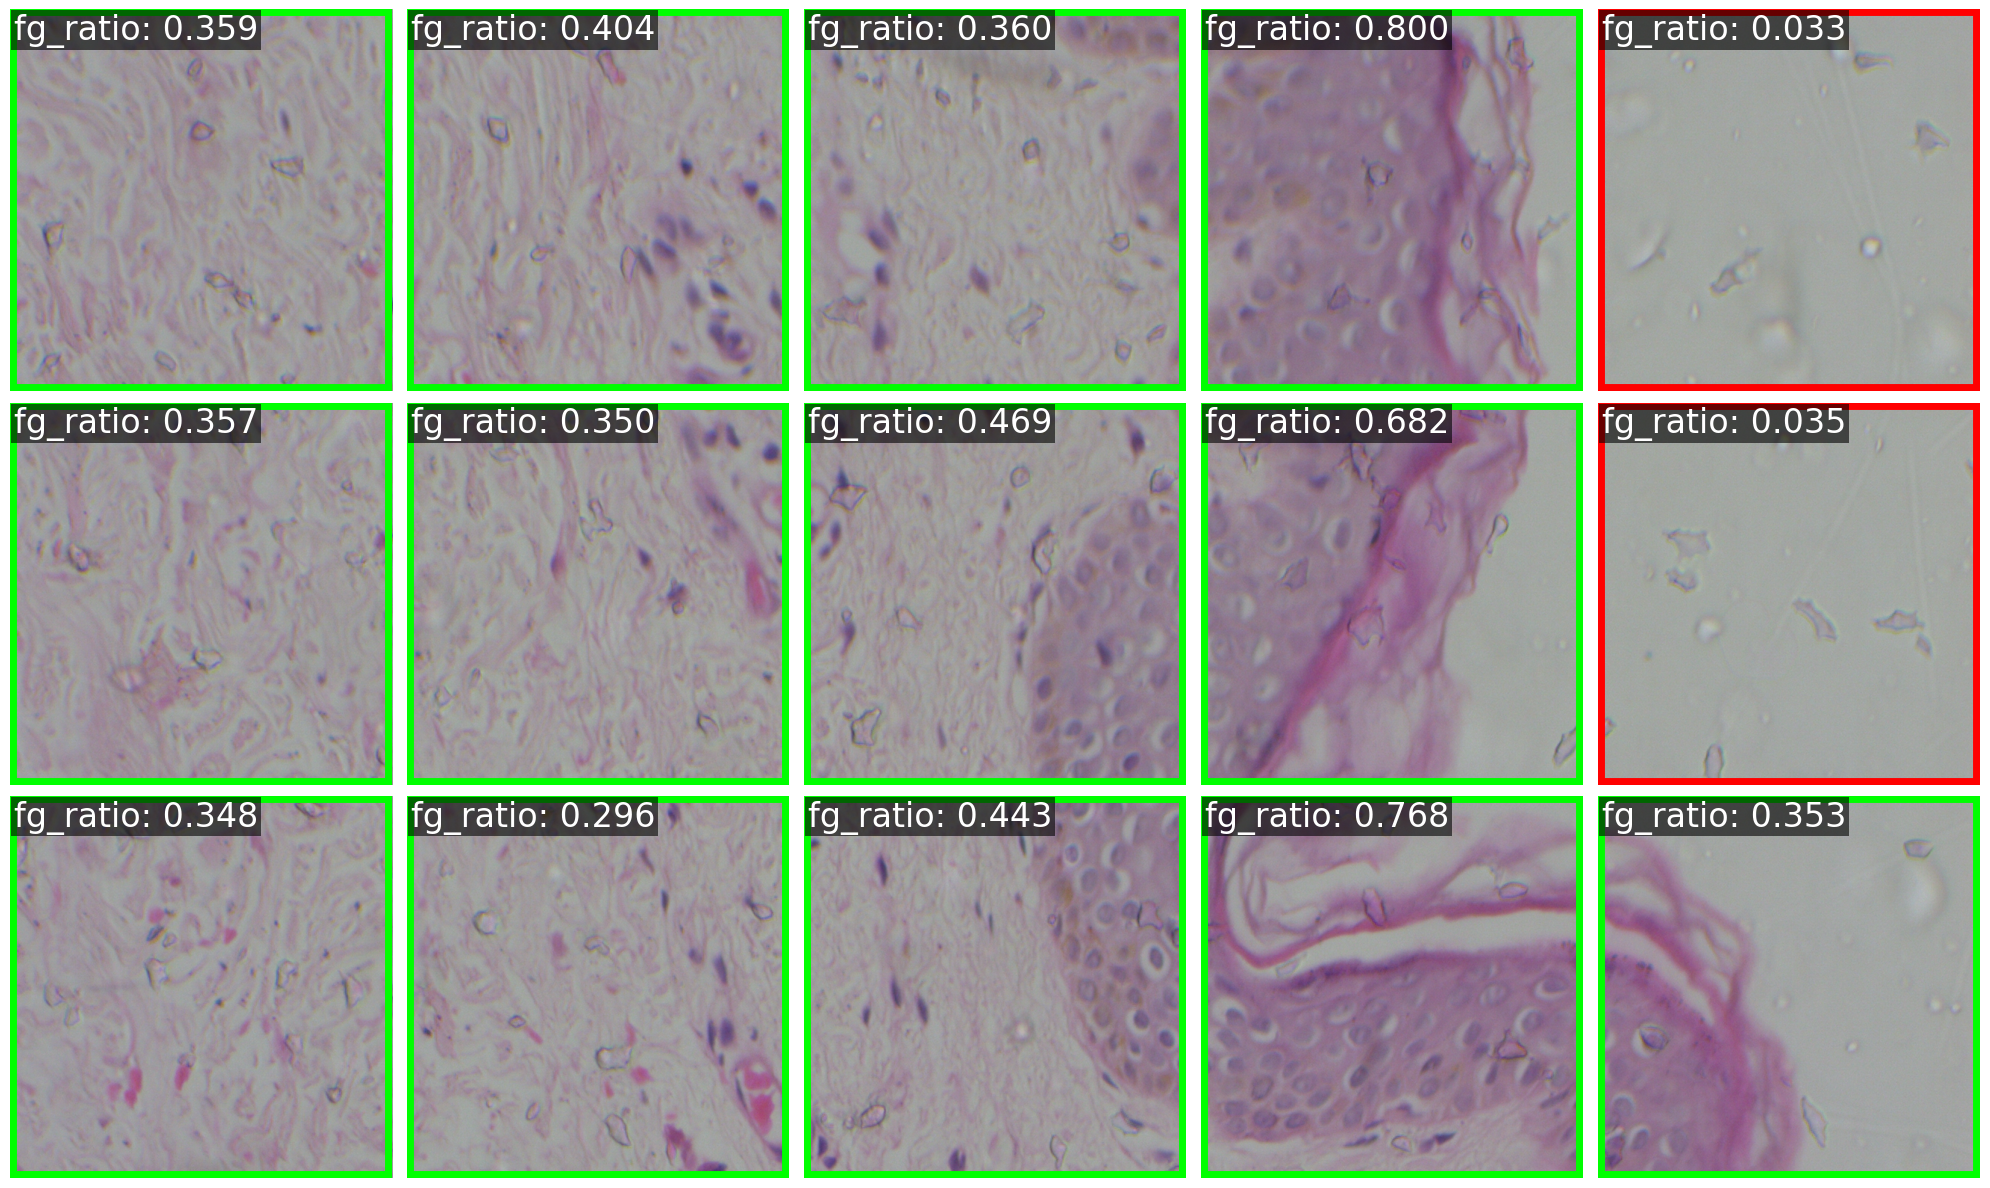
\includegraphics[width=0.8\linewidth]{HSV_Ratio.png}
    \caption{Different foreground ratios for patches of a sample tif image}
    \label{fig:HSV_Ratio}
\end{figure}

\subsection{Model Architecture and Training Protocol}

\subsubsection{Backbone Selection and Hyperparameter Optimization}
To determine the optimal feature extractor for histopathological classification, we investigated a convolutional neural network architecture: ResNet50. To ensure robust convergence and generalization, we automated the model selection and hyperparameter tuning process using the Optuna framework. We employed a Tree-structured Parzen Estimator (TPE) sampler with a Median Pruner to efficiently search the hyperparameter space. The optimization process consisted of 30 trials performed on a stratified 15\% subset of the training data. The search space included learning rates ($10^{-5}$--$10^{-3}$), weight decay ($10^{-6}$--$10^{-3}$), dropout ratios (0.1--0.4), and batch sizes of $\{8, 16\}$. As shown in Table \ref{tab:hyperparams}, ResNet50 was identified as the superior architecture for both magnification levels. The tuning process achieved a best validation accuracy of 70.36\% for 10x and 73.91\% for 20x.

\begin{table}[H]
\caption{Optimal Hyperparameters Selected via Optuna}
\begin{center}
\begin{tabular}{lcc}
\toprule
\textbf{Hyperparameter} & \textbf{10$\times$ Magnification} & \textbf{20$\times$ Magnification} \\
\midrule
Architecture & ResNet50 & ResNet50 \\
Learning Rate & $3.95 \times 10^{-5}$ & $3.22 \times 10^{-5}$ \\
Weight Decay & $9.84 \times 10^{-4}$ & $2.13 \times 10^{-4}$ \\
Dropout Rate & 0.40 & 0.26 \\
Batch Size & 8 & 8 \\
\midrule
\textbf{Best Val. F2-Score} & \textbf{0.6412} & \textbf{0.7398} \\
\bottomrule
\end{tabular}
\label{tab:hyperparams}
\end{center}
\end{table}

\subsubsection{Metric Selection and Checkpointing}
Given the critical nature of cancer diagnosis, minimizing False Negatives is paramount. Consequently, we prioritized Sensitivity (Recall) over raw accuracy during the training process. Model checkpointing was governed by the F2-score, which weighs recall twice as heavily as precision:

\begin{equation}
    F_2 = (1 + 2^2) \cdot \frac{\text{Precision} \cdot \text{Recall}}{(2^2 \cdot \text{Precision}) + \text{Recall}}
\label{eq:f2_score}
\end{equation}

The models saved for final testing were those that achieved the highest F2-score on the validation set (0.6412 for 10x and 0.7398 for 20x), ensuring the system is biased towards detecting malignant cases.

\subsubsection{Training Strategy}
The models were trained using the AdamW optimizer with Automatic Mixed Precision (AMP) to optimize GPU memory usage. To address the inherent class imbalance between Mycosis Fungoides (MF) and Non-MF samples, we utilized a Weighted Cross-Entropy Loss, where class weights were assigned inversely proportional to their frequency in the training set.

\subsubsection{Validation Protocol and Aggregation Performance}
To bridge the gap between model training and clinical utility, we adopted a hierarchical evaluation strategy. While the models were optimized using patch-level objectives, the final diagnostic performance was assessed at the patient level on a held-out validation cohort comprising 35 patients (totaling 8,077 patches at 10$\times$ and 15,996 patches at 20$\times$). Our experiments demonstrated that \textit{Mean Aggregation} significantly enhanced diagnostic performance. For the 10$\times$ model, aggregating predictions improved the F2-score from 0.7134 (patch-level) to 0.8482 (patient-level), achieving a balanced sensitivity and specificity of 86.36\%. Similarly, the 20$\times$ model achieved a patient-level ROC-AUC of 0.7972, up from 0.7420 at the patch level. These results confirm that utilizing the collective signal from multiple tissue regions mitigates local ambiguities, justifying the adoption of mean aggregation for the final pipeline.

\subsection{Patient-Level Prediction via Mean Aggregation}
Model inference was initially performed at the patch level. To obtain clinically meaningful predictions at the patient level, patch-level probabilities corresponding to the same patient were aggregated using mean aggregation. Given a patient $p$ with $N_p$ patches and predicted probabilities $\{s_1, s_2, \ldots, s_{N_p}\}$, the patient-level score $S_p$ was computed as:
\begin{equation}
S_p = \frac{1}{N_p} \sum_{i=1}^{N_p} s_i
\end{equation}

Mean aggregation was selected due to its simplicity, robustness to noise, and interpretability in a clinical context.

\subsection{Multi-Magnification Fusion Strategy}

\subsubsection{Late Fusion Approach}
To integrate complementary diagnostic features captured at different scales, we employed a \textit{late fusion} strategy. Unlike early fusion, which concatenates feature vectors prior to classification, late fusion aggregates the probabilistic predictions of independent models. This approach allows each network to specialize in the specific histological patterns visible at its respective magnification—capturing architectural disarray at $10\times$ and cellular atypia at $20\times$—without the risk of feature-space contamination.

\subsubsection{Weighted Score Aggregation and Clinical Justification}
In clinical practice, dermatopathologists employ a multi-scale workflow: they initially scan tissue at low magnification to identify broad architectural abnormalities (e.g., epidermotropism) before zooming in to high magnification to assess individual cellular atypia. Our late-fusion approach mimics this workflow by integrating both perspectives. Let $S_{p}^{10}$ and $S_{p}^{20}$ denote the mean-aggregated patient-level probabilities obtained from the $10\times$ and $20\times$ models, respectively. The final fused diagnostic score $S_{p}^{fused}$ was computed as a linear combination:
\begin{equation}
S_{p}^{fused} = \alpha S_{p}^{10} + (1 - \alpha) S_{p}^{20}
\end{equation}
where $\alpha \in [0, 1]$ represents the fusion weight governing the contribution of the $10\times$ model.

\subsubsection{Optimization of Fusion Weight}
The optimal weight $\alpha$ was determined empirically by minimizing the Brier Score on the validation set. The optimization consistently assigned a higher weight to the $10\times$ model ($\alpha > 0.5$). Clinically, this is both acceptable and expected; Mycosis Fungoides is heavily defined by its architectural distribution across the epidermis and dermis. Therefore, the $10\times$ spatial context appropriately drives the primary diagnostic probability, while the $20\times$ model acts as a secondary calibrator that refines the prediction based on cellular features. This multi-scale synergy yields a more robust and clinically aligned outcome than relying on a single field of view. 

As illustrated in Figure \ref{fig:fusion_analysis}, we performed a grid search for $\alpha$ with a step size of 0.05. The analysis revealed a convex optimization landscape (top-left panel), with the global minimum Brier Score achieved at $\alpha = 0.65$. This weighting suggests that the architectural context provided by the $10\times$ magnification was slightly more predictive than the cellular details at $20\times$ for this cohort. Consequently, $\alpha = 0.65$ was adopted for all subsequent evaluations, yielding a stable balance between sensitivity (0.86) and specificity.

\begin{figure}[H]
    \centering
    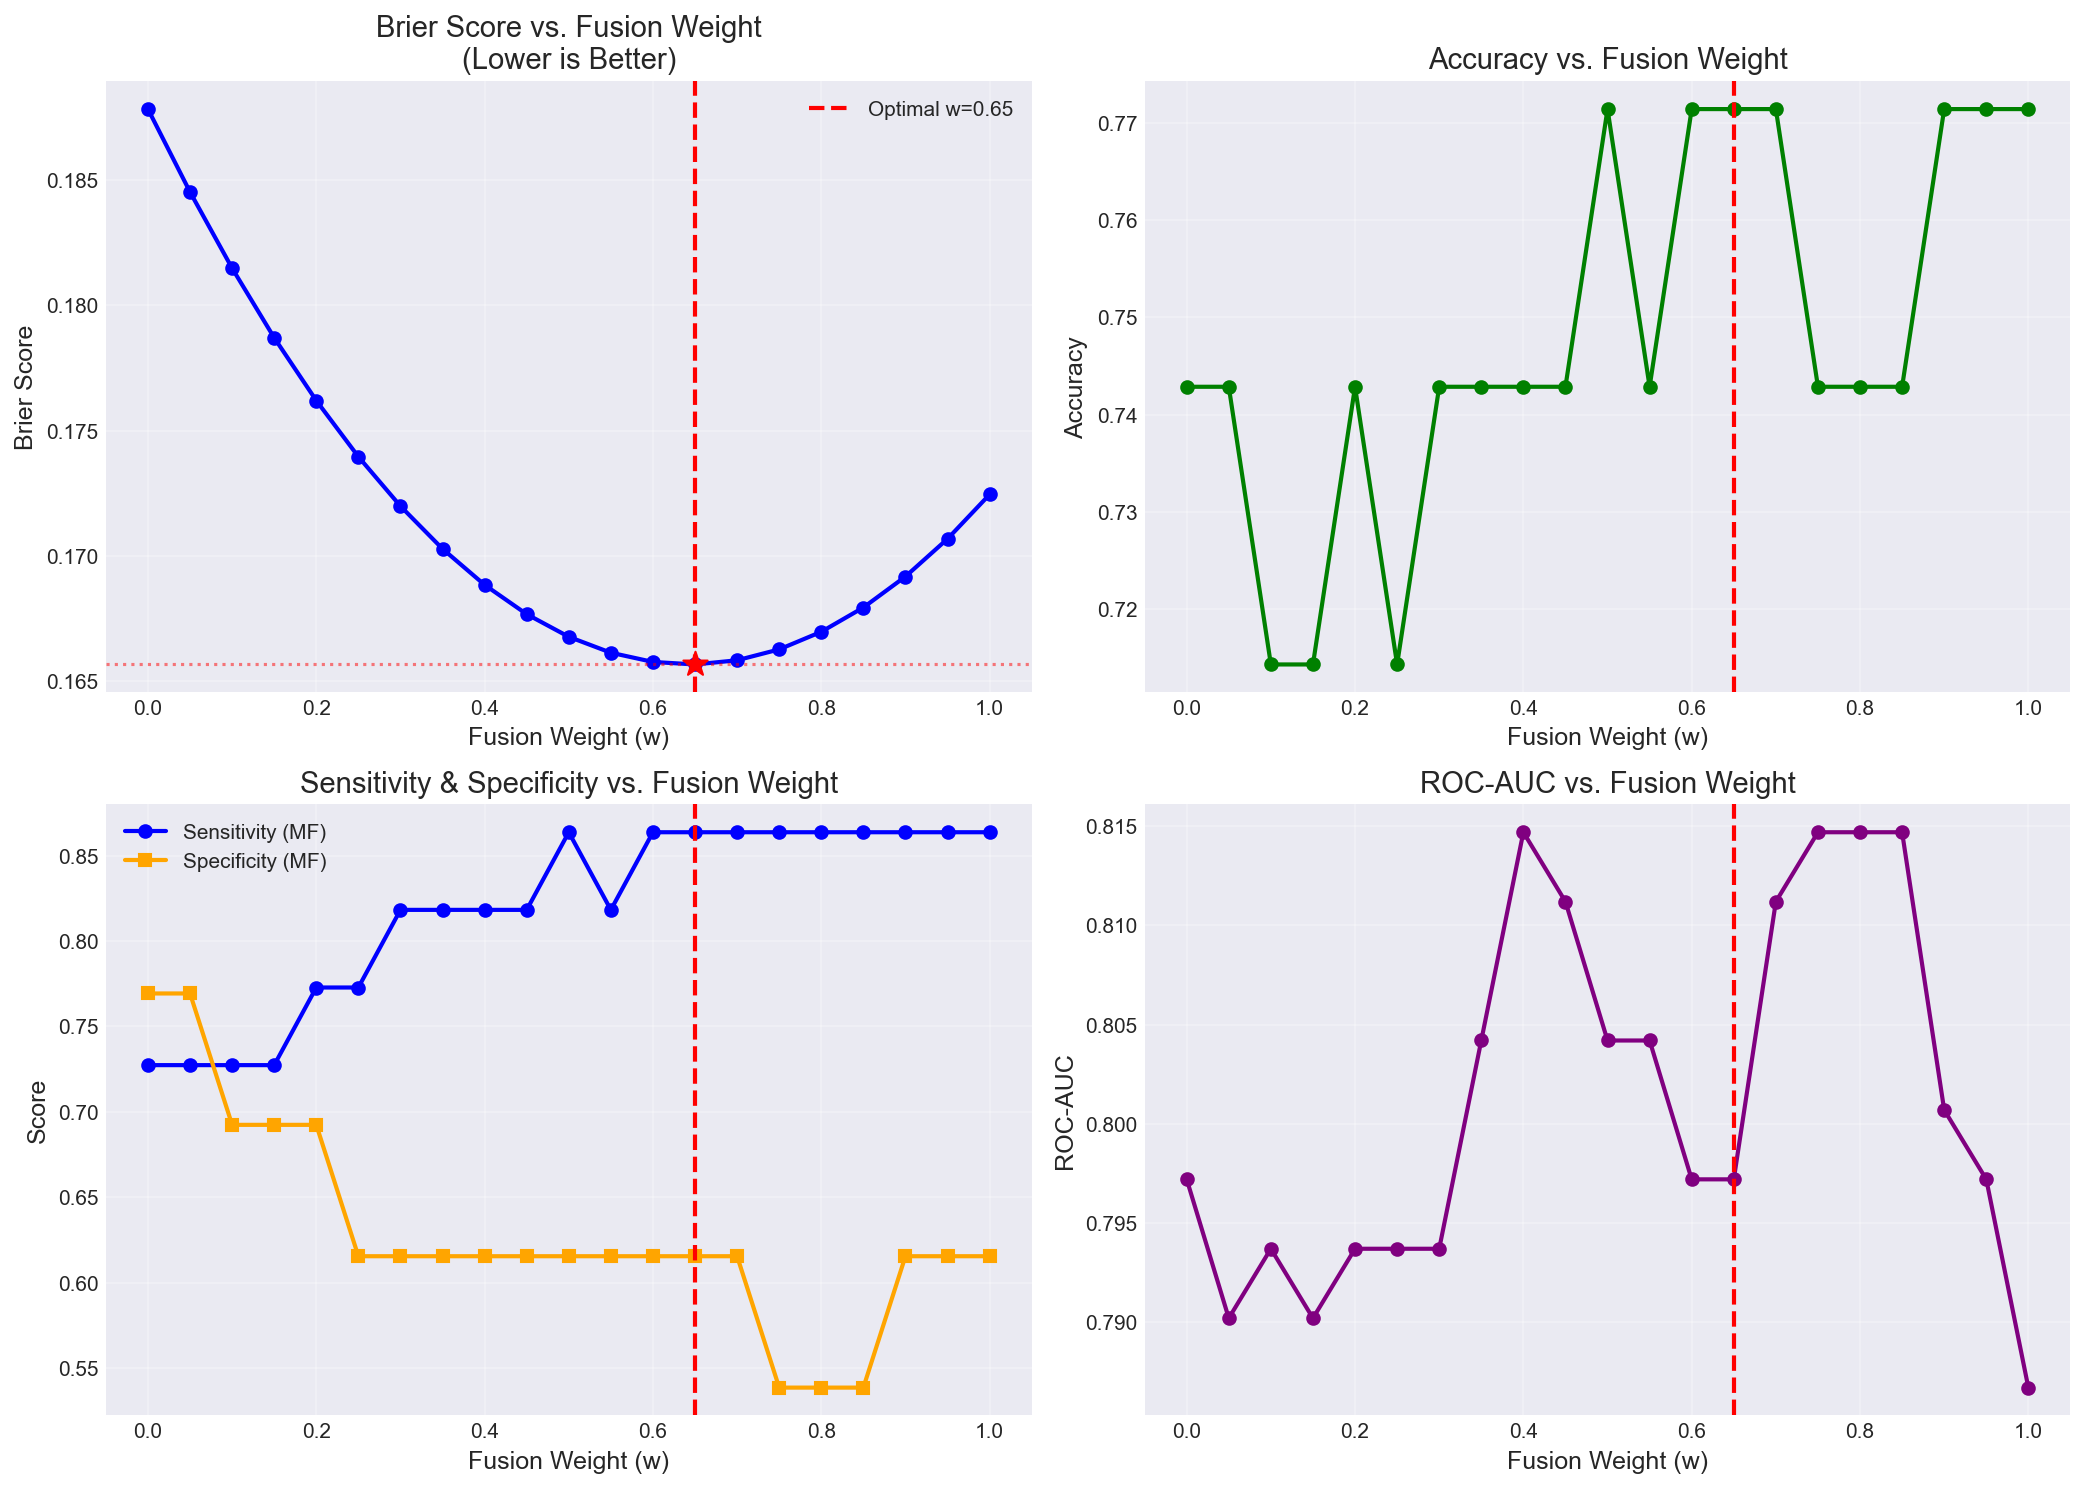
\includegraphics[width=0.8\linewidth]{fusion_weight_analysis.png}
    \caption{Optimization of the multi-magnification fusion weight ($\alpha$). The top-left panel demonstrates that the lowest Brier Score (indicating optimal calibration) is achieved at $\alpha=0.65$. The remaining panels illustrate the corresponding trade-offs in Accuracy, Sensitivity/Specificity, and ROC-AUC, confirming that this weight maintains high sensitivity while maximizing predictive reliability.}
    \label{fig:fusion_analysis}
\end{figure}

% =====================
% 4. Results
% =====================
\section{Results}

The proposed deep learning framework was evaluated on a held-out test set of 35 patients, comprising 8,077 patches at 10$\times$ magnification and 15,996 patches at 20$\times$ magnification. As summarized in Table \ref{tab:results}, the system achieved a maximum magnification-level accuracy of 77.14\% and an F$_2$-score of 84.82\% using the late-fusion model.

\begin{table}[htbp]
\caption{Quantitative Performance Summary (Test Set, N=35)}
\label{tab:results}
\centering
\renewcommand{\arraystretch}{1.2}
\setlength{\tabcolsep}{6pt} 
\begin{tabular}{l c c c}
\toprule
 & \textbf{10$\times$ Model} & \textbf{20$\times$ Model} & \textbf{Late Fusion} \\
\midrule
Accuracy & \textbf{0.7714} & 0.7429 & \textbf{0.7714} \\
F$_2$-Score & \textbf{0.8482} & 0.7477 & \textbf{0.8482} \\
Sensitivity & \textbf{0.8636} & 0.7273 & \textbf{0.8636} \\
Specificity & 0.8636 & 0.7273 & 0.6154 \\
ROC-AUC & 0.7867 & \textbf{0.7972} & \textbf{0.7972} \\
\bottomrule
\end{tabular}
\end{table}

\subsection{Patient-Level Aggregation Benefits}
A key finding of this study is the significant performance gain achieved through patient-level aggregation. As illustrated in the comprehensive dashboard (Fig. \ref{fig:comprehensiveMetrics}), every metric improved when moving from patch-level predictions to patient-level consensus.

\begin{figure}[H]
    \centering
    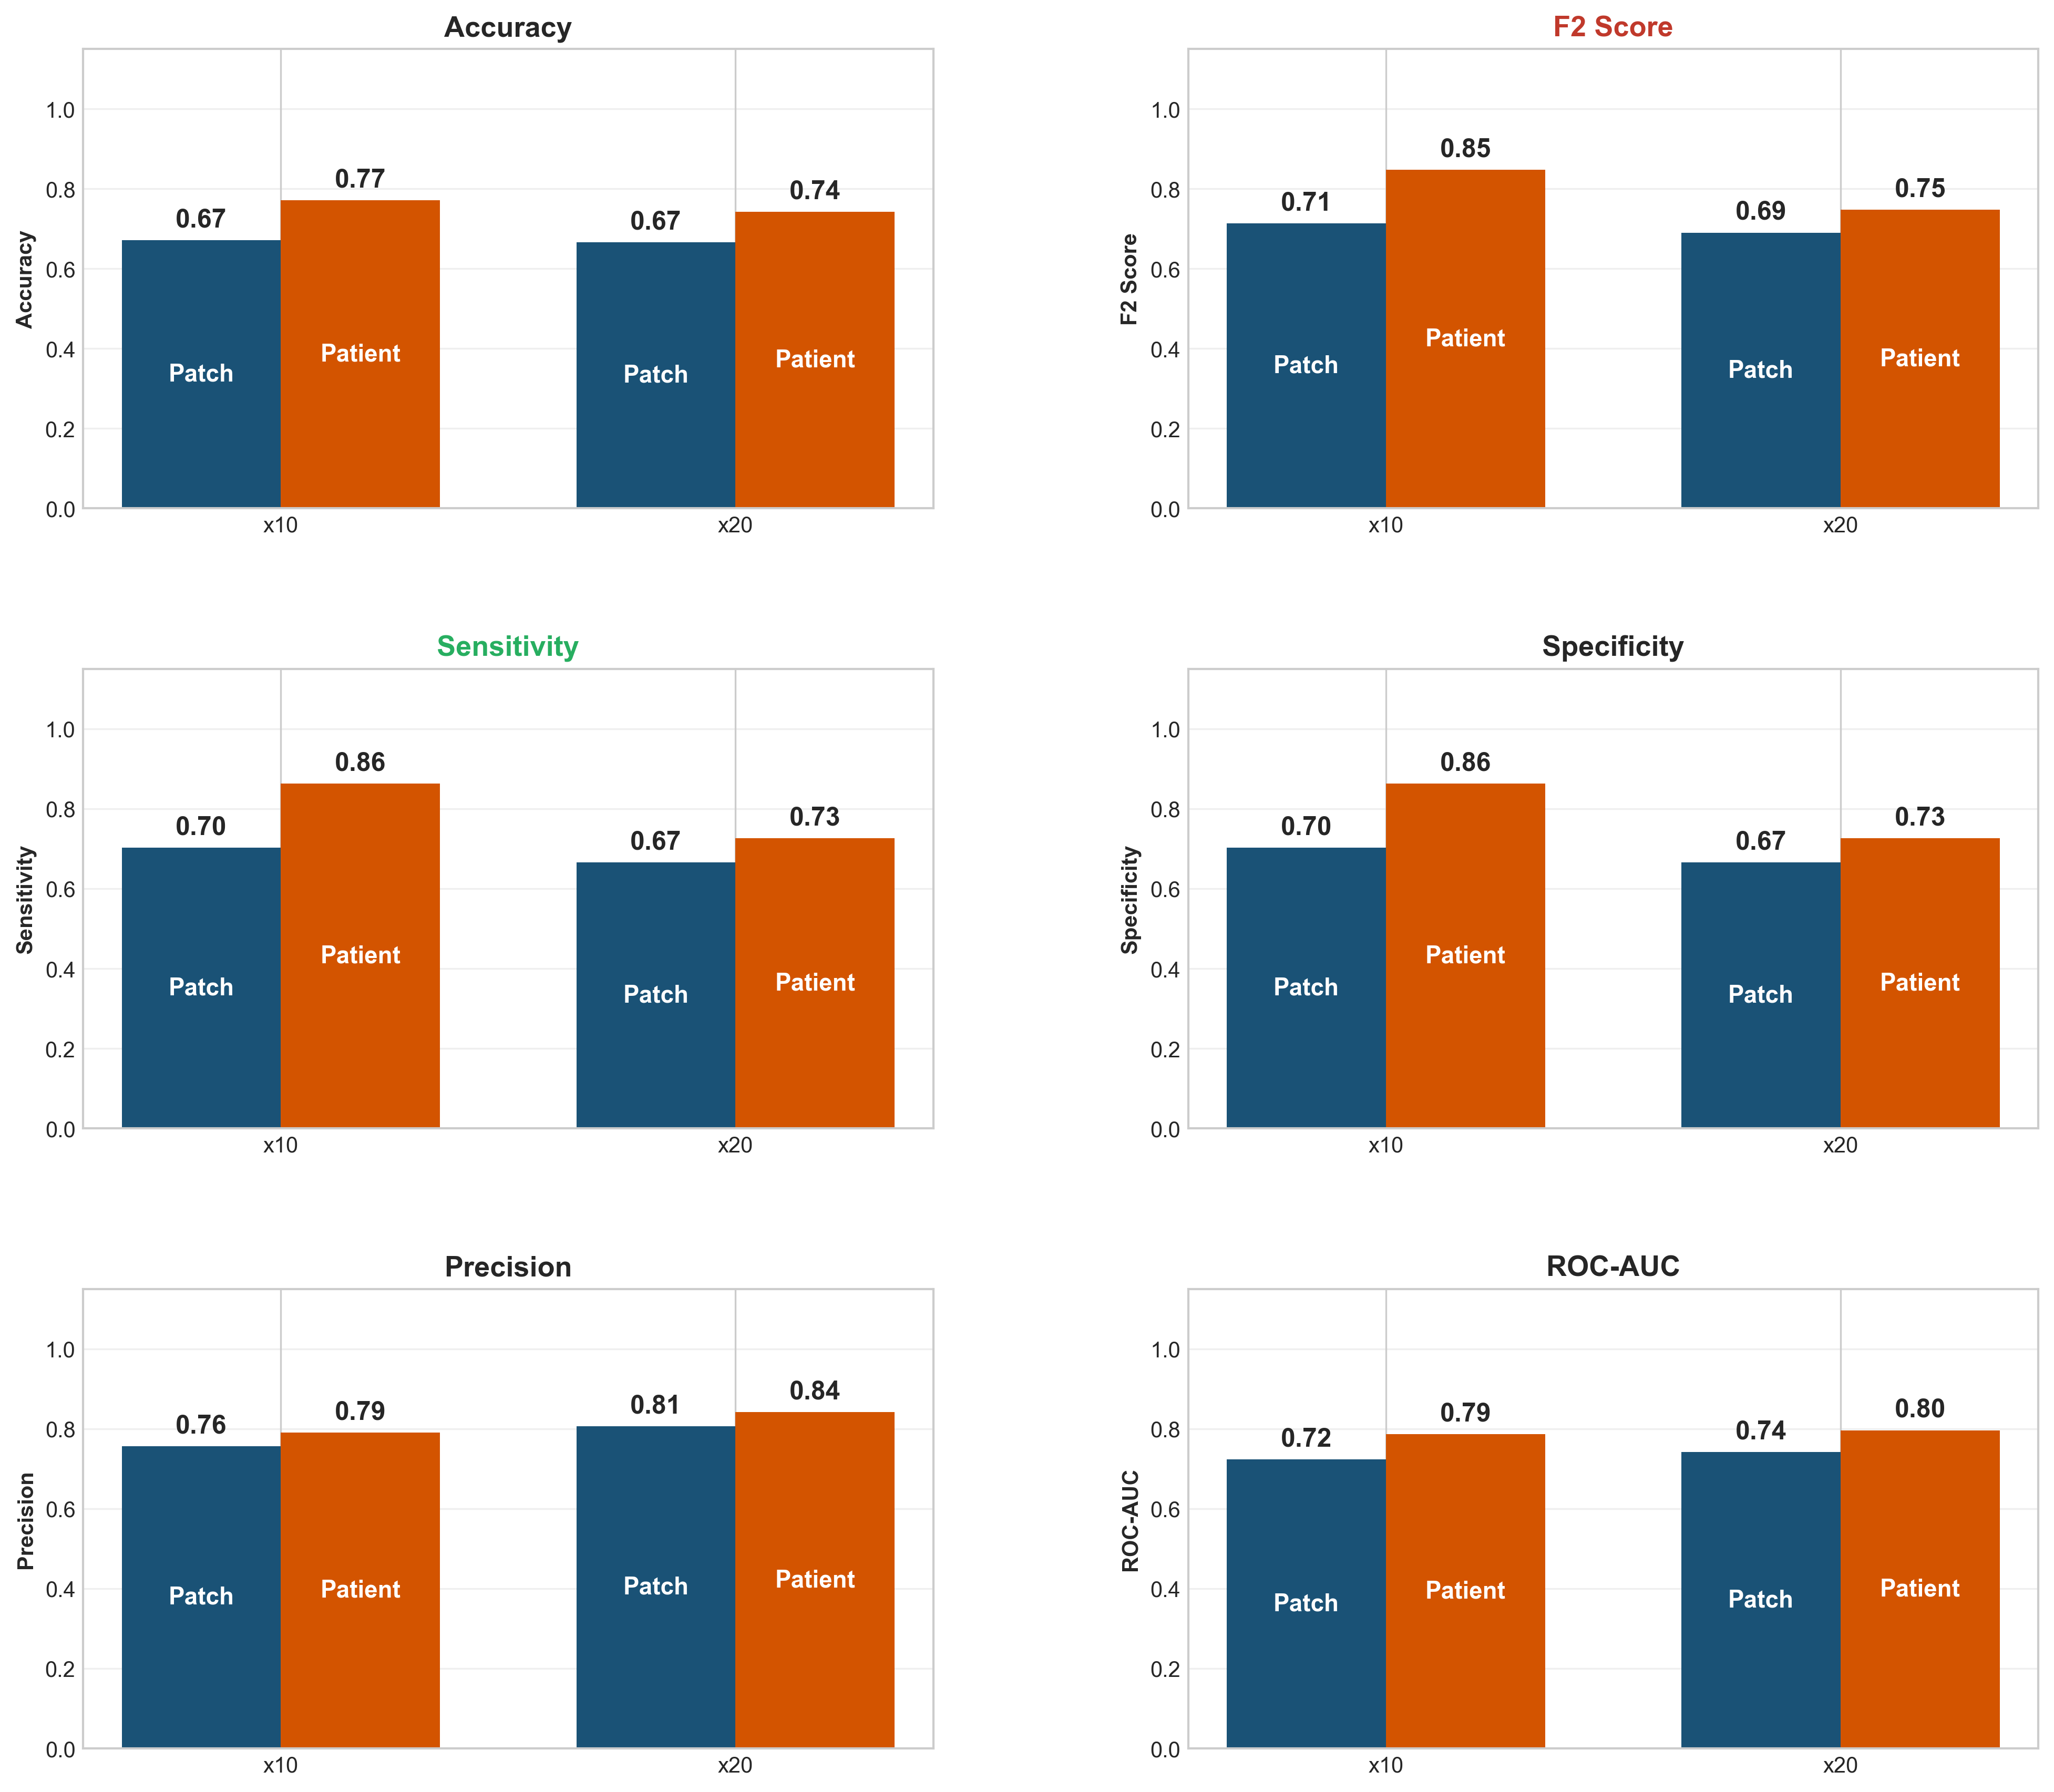
\includegraphics[width=0.8\linewidth]{Comprehensive Metrics Dashboard.png}
    \caption{Comprehensive Performance Dashboard. A side-by-side comparison of patch-level (dark blue) vs. patient-level (dark orange) metrics across both magnifications.}
    \label{fig:comprehensiveMetrics}
\end{figure}

\begin{figure}[H]
    \centering
    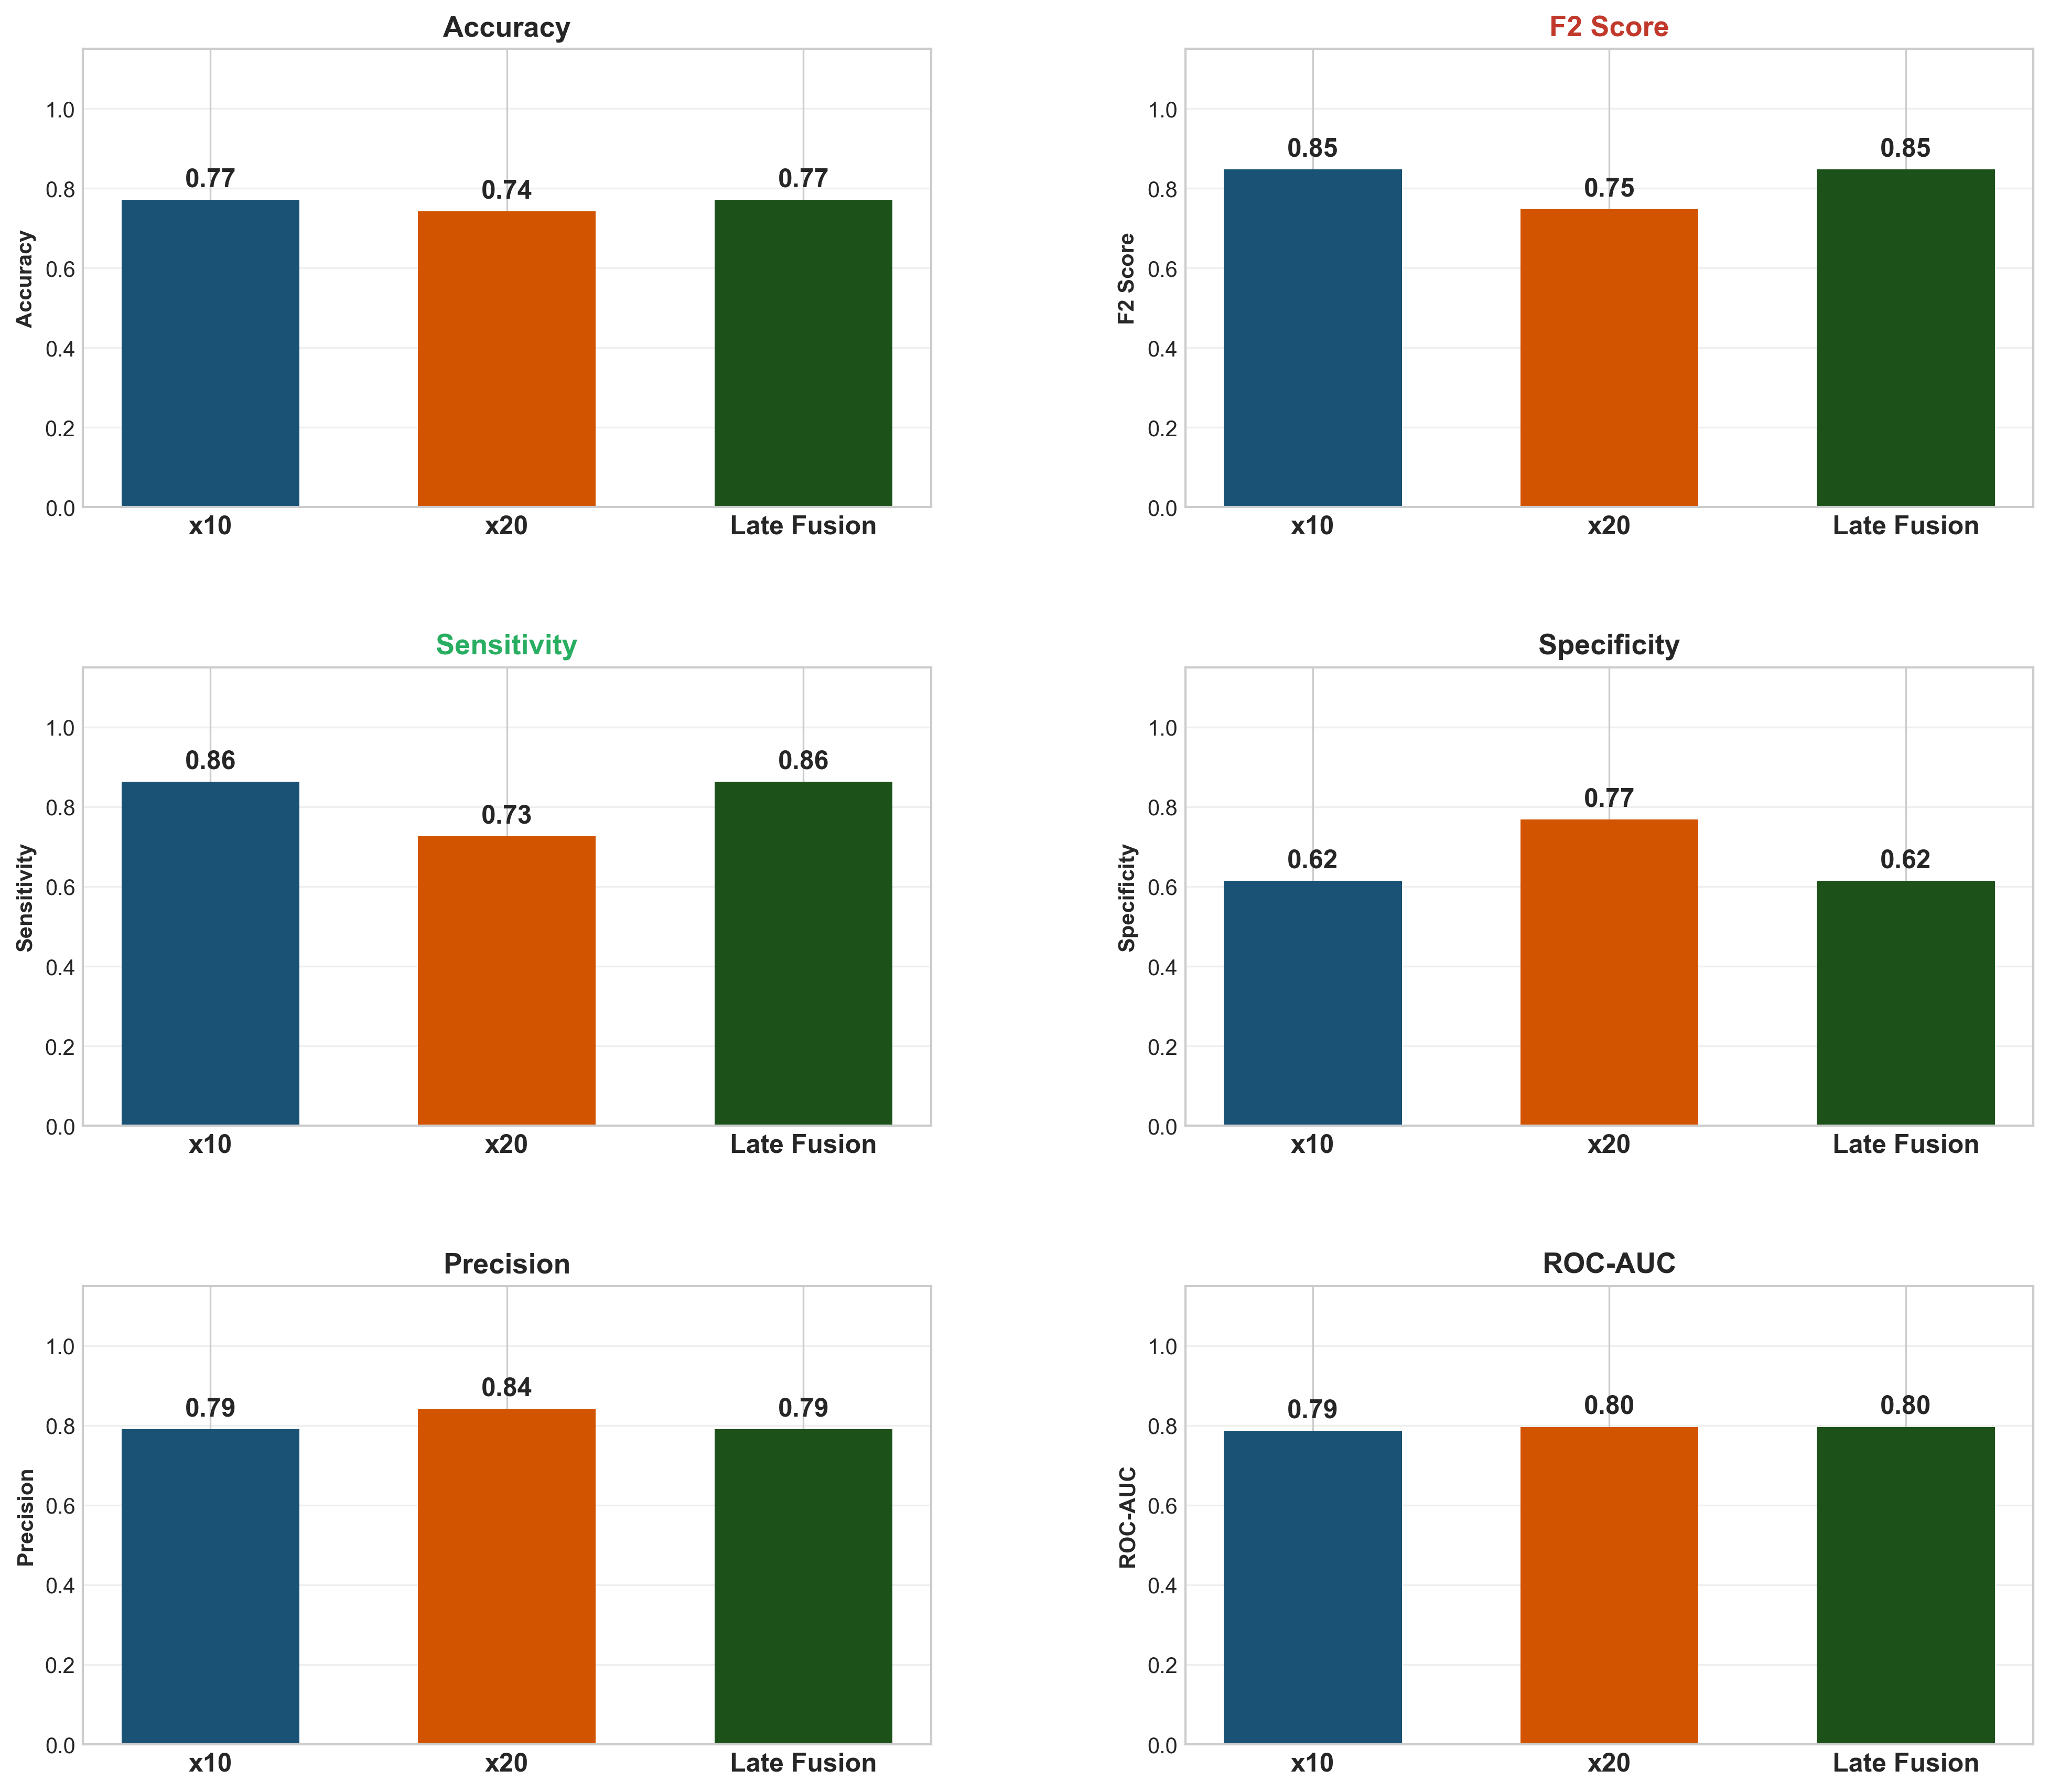
\includegraphics[width=0.8\linewidth]{Late_fusion_dashboard.png}
    \caption{Late fusion model performance comparing individual magnification models (10$\times$, 20$\times$) against the fused multi-scale approach. Late fusion combines predictions from both magnifications to leverage complementary information captured at different scales.}
    \label{fig:aggregation_comparison}
\end{figure}

This improvement is further detailed in the comparative performance dashboard (Fig. \ref{fig:aggregation_comparison}), which illustrates the metric shifts across magnifications and aggregation levels. The transition from patch-level to patient-level inference yields substantial gains across the board. Notably, the late fusion strategy successfully synthesizes the diagnostic strengths of both individual models: it matches the peak sensitivity (0.8636) and F$_2$-score (0.8482) of the 10$\times$ patient-level model, while simultaneously achieving the highest ROC-AUC (0.7972) alongside the 20$\times$ model. Although this multi-scale fusion incurs a trade-off by lowering specificity (0.6154), it effectively maximizes the detection of True Positives. In the clinical context of Mycosis Fungoides screening, prioritizing sensitivity over specificity ensures that ambiguous but potentially malignant cases are not missed, confirming the robustness of integrating global slide context across multiple magnifications.

\subsection{Sensitivity and Clinical Relevance}
Given the clinical imperative to minimize missed diagnoses, we prioritized the F$_2$-score (which emphasizes recall). The 10$\times$ model achieves a superior F$_2$-score of 0.848 compared to 0.748 for the 20$\times$ model. This suggests that architectural changes visible at lower magnification are highly indicative of MF. This result is corroborated by the Receiver Operating Characteristic (ROC) and Precision-Recall (PR) curves (Fig. \ref{fig:roc} and Fig. \ref{fig:pr}). The patient-level curves (solid lines) consistently envelop the patch-level curves (shaded areas), demonstrating superior discriminatory power across all decision thresholds.

\begin{figure}[H]
    \centering
    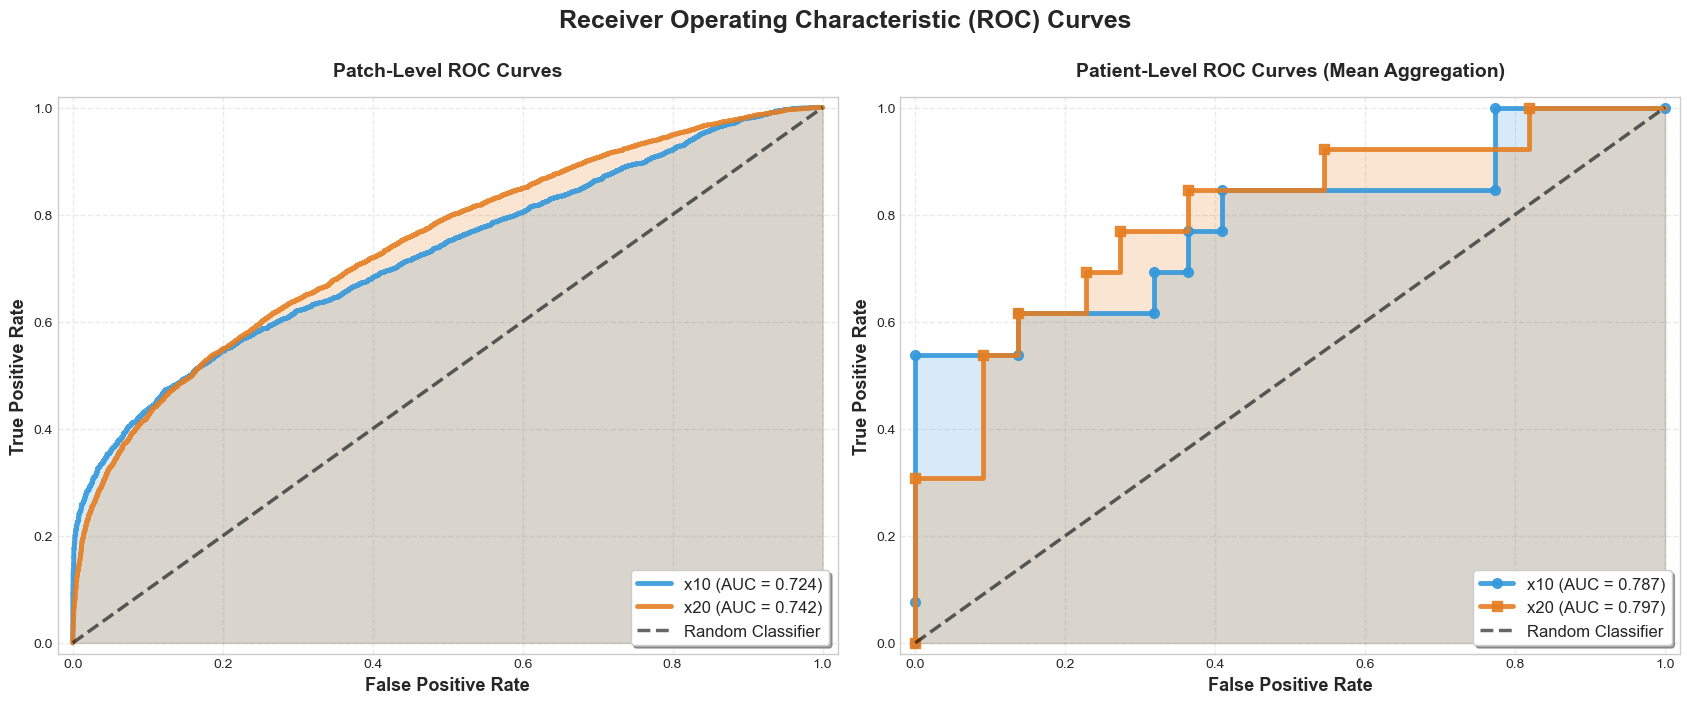
\includegraphics[width=0.8\linewidth]{ROC Graphs.png}
    \caption{Receiver Operating Characteristic (ROC) Curves. The "step-like" nature of the patient-level curves is due to the discrete number of test patients (N=35), yet they show a clear improvement in Area Under the Curve (AUC) compared to patch-level inference.}
    \label{fig:roc}
\end{figure}

\begin{figure}[H]
    \centering
    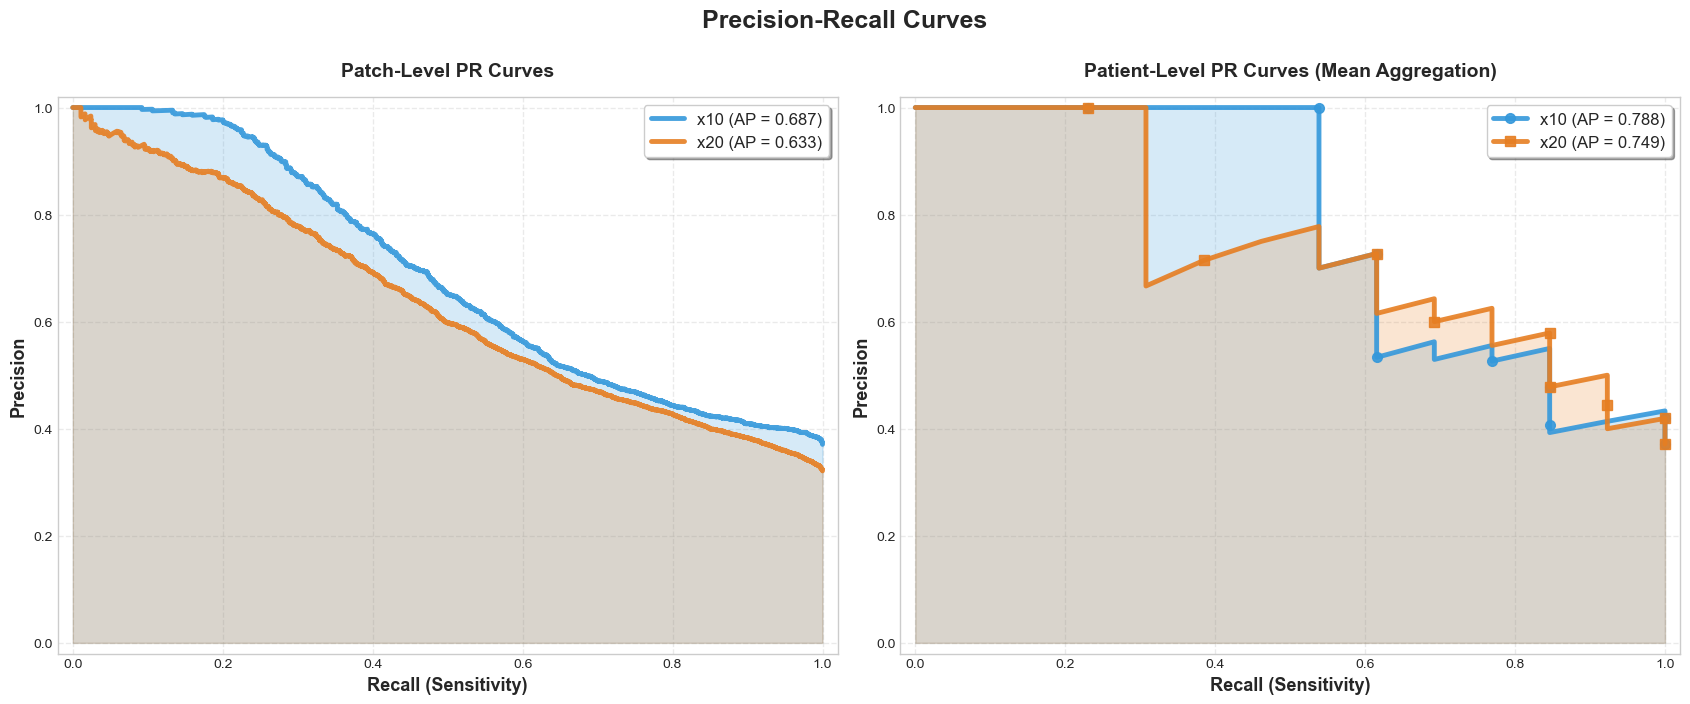
\includegraphics[width=0.8\linewidth]{Precision Recall Curves.png}
    \caption{Precision-Recall Curves. The dominance of the patient-level curves (solid lines) confirms that the model maintains high precision even at higher recall levels, a critical trait for a screening tool.}
    \label{fig:pr}
\end{figure}

% =====================
% 6. Discussion
% =====================
\section{Discussion}
\subsection{Architectural vs. Cellular Features and Patch Resolution}
A counter-intuitive finding of this study is the superior performance of the 10$\times$ model (F$_2$=0.848) compared to the 20$\times$ model (F$_2$=0.748). In histopathology, higher magnification typically yields better resolution of cellular atypia. However, Mycosis Fungoides is largely defined by architectural patterns, such as the distribution of lymphocytes along the dermo-epidermal junction (epidermotropism) and the formation of Pautrier's microabscesses. Our results suggest that the wider field of view at 10$\times$ captures these broad architectural context cues more effectively than the granular but narrow view of 20$\times$. 

This phenomenon is likely exacerbated by the fixed patch size of $512 \times 512$ pixels used in this study. At 10$\times$, a $512 \times 512$ patch covers a sufficient physical area to encapsulate the dermo-epidermal junction and surrounding infiltrate. Conversely, at 20$\times$, the same pixel dimensions cover a significantly smaller physical area, potentially fragmenting these critical architectural features. While the 10$\times$ magnification proved optimal for this specific patch configuration, future work must explore larger patch sizes or multi-scale inputs to fully leverage the cellular details available at 20$\times$ magnification.

\subsection{The Necessity of Whole-Slide Context}
The success of the patient-level aggregation strategy highlights the diffuse nature of Mycosis Fungoides. Because MF features are rarely restricted to a few isolated "hotspots" and are instead spread subtly across the tissue, relying on the collective signal of the entire sample is crucial. By utilizing mean aggregation, the model effectively integrates the probabilistic signal from all extracted patches. This approach acts as a digital analog to a pathologist comprehensively scanning the whole tissue slide before making a final diagnostic decision, ensuring that widespread, subtle architectural cues are fully leveraged.

\subsection{Benchmarking and Clinical Reality}
While our deep learning framework demonstrates high diagnostic potential, it is crucial to acknowledge that diagnosing Mycosis Fungoides solely from histopathological images is a simplified proxy for clinical reality. In practice, dermatologists and pathologists rely on a multimodal synthesis of visual data, patient history, and clinical presentation (e.g., lesion morphology, duration) to render a definitive diagnosis. The reliance on image data alone in this study likely imposes a performance ceiling; we hypothesize that integrating tabular clinical metadata in future iterations will significantly enhance diagnostic precision and reduce false positives.

Despite this limitation, our model's performance is highly competitive with recent state-of-the-art benchmarks. Doeleman et al. \cite{Doeleman2024-MF} compared a weakly supervised deep learning model against three expert pathologists. They reported that their highest performance was achieved at $200\times$ magnification ($0.50$ $\mu$m/pixel), yielding a mean Area Under the Curve (AUC) of $0.827 \pm 0.044$ and a mean balanced accuracy of $76.2 \pm 3.9\%$. In comparison, our $10\times$ model achieved a patient-level accuracy of $77.1\%$ and a sensitivity of $86.4\%$. Notably, our framework effectively matches the accuracy of expert pathologists reported in \cite{Doeleman2024-MF}.

% =====================
% 7. Conclusion
% =====================
\section{Conclusion}
This work presents a clinically viable and computationally efficient deep learning framework for the automated screening of Mycosis Fungoides. By rigorously optimizing a ResNet50 backbone and employing a patient-level fusion strategy, we achieved a diagnostic sensitivity of 86.4\% and an ROC-AUC of 0.79 on an independent validation cohort. Our results demonstrate that effective diagnosis does not necessarily require high-magnification whole-slide imaging. Instead, the architectural patterns visible at lower resolutions are sufficiently discriminative for reliable screening. This finding has significant implications for global health equity, as it reduces the dependency on high-end digitization hardware. Our key contributions include:

\begin{enumerate}
    \item \textbf{Efficient Initial Triage Tool:} We demonstrated that low magnification (10$\times$) effectively captures broad architectural features, yielding competitive accuracy for initial MF screening. While we acknowledge that higher magnifications remain clinically necessary for the definitive differential diagnosis between MF and morphologically similar inflammatory dermatoses, our 10$\times$ framework significantly reduces computational overhead. This makes the system fast to run and highly suitable as an accessible, first-pass triage tool in resource-constrained settings.
    \item \textbf{Robustness Without Clinical Metadata:} We established that deep learning models can achieve high sensitivity solely based on histopathological features. While real-world diagnosis benefits from clinical history, our model serves as a powerful standalone triage tool for unannotated archival data or blind review scenarios.
    \item \textbf{Multi-Scale Patient-Level Late Fusion:} We designed a late-fusion aggregation protocol that integrates predictions across multiple magnifications. By systematically combining the broad architectural context captured at 10$\times$ with the cellular-level signals from the 20$\times$ model, our patient-level consensus approach achieved an optimal balance of performance. This fusion strategy maintained the high sensitivity of the low-power model while matching the superior discriminatory power (ROC-AUC) of the high-power model, confirming the necessity of multi-scale analysis in digital pathology.
\end{enumerate}

% =====================
% 8. Future Work
% =====================
\section{Future Work}
To evolve this framework from a promising prototype into a robust clinical decision-support system, future research will address four critical limitations:

\begin{enumerate}
    \item \textbf{Optimization of 20$\times$ Patch Resolution:} The current underperformance of the 20$\times$ model relative to the 10$\times$ model contradicts histopathological intuition, where higher magnification typically yields richer cellular detail. We hypothesize that the fixed $512 \times 512$ patch size captures insufficient architectural context at high magnification. Future experiments will systematically evaluate larger patch dimensions and multi-scale inputs for the 20$\times$ classifier, with the expectation that optimizing this field of view will allow it to surpass the 10$\times$ model's accuracy.
    \item \textbf{Multimodal Integration:} Diagnosing Mycosis Fungoides purely from imagery is clinically incomplete. We plan to integrate the visual backbone with a tabular data branch processing patient metadata (e.g., age, gender, lesion duration, and symptoms). This multimodal fusion is expected to significantly enhance specificity by mimicking the comprehensive work-up performed by dermatologists.
    \item \textbf{Stain Normalization and Augmentation:} To ensure the model generalizes across different laboratories and scanners, we will implement rigorous stain normalization techniques (e.g., Macenko \cite{macenko2009} or Vahadane \cite{vahadane2016_stainnorm} methods) in the preprocessing pipeline. This will mitigate the impact of color variations in H\&E staining that can currently confound the classifier.
\end{enumerate}

\bibliographystyle{splncs04}
\bibliography{references}

\end{document}